\subsection{Compartmentalization}
%objective
%I estimated the degree of compartmentalization calculating the relative area or volume of expression of genes during development.
%My intention here was not to focus on individual genes, but to get a global overview of the embryo compartmentalization and differentiation processes based on expression data of thousands of genes, i.e., using a statistical approach.
%
%One would expect, and it has been implicitly assumed \citep{Carroll2001} \citep{Davidson2001} that the compartmentalization of the embryo (as I measure it here) increases during development.
%However, the specific temporal dynamics of this increase in any species is not known. Neither is clear if the dynamics should be similar for different species, or for different groups of genes.

As the development of \textit{Ciona} and \textit{Drosophila} are very different and it would be impossible to compare them stage-by-stage, I focused here in three major developmental periods: pre-gastrula, gastrula, and post-gastrula stages. These periods are easily recognizable in both species facilitating the comparative analysis.

%results
I found that in both species, the relative area or volume decreased in a non-linear way (see Fig. \ref{fig:Art-I-3measures} and Fig. \ref{fig:Art-II-3measures}). 
However, the timing of the major decrease was different.
In \textit{Drosophila} the major decrease occurred at very early development, from maternal to early gastrula stage (Fig. \ref{fig:Art-I-3measures}).
Practically half of the genes in follows this decrease pattern: 46\% of the genes were characterized as having a non-linear decrease in their relative area.
In contrast, in \textit{Ciona} the volume of expression decreases mostly after gastrulation (between the 112-cell and the early tailbud stage).
However less dramatic, I found significant differences between the 32-cell and 64-cell stages, and between the 64-cell and 112-cell stages.

%%%%%%%%%%%%%%%%%%%%%%%%%%%%%%%%%%%%%%%%%%%%%%%%%%%%%%%%%%%%%%%%%%%%%%%%%%%%%%%%%%%%%%%%%%%%%%%%%%%%%%%%%%%%%%
\begin{figure}[b]
  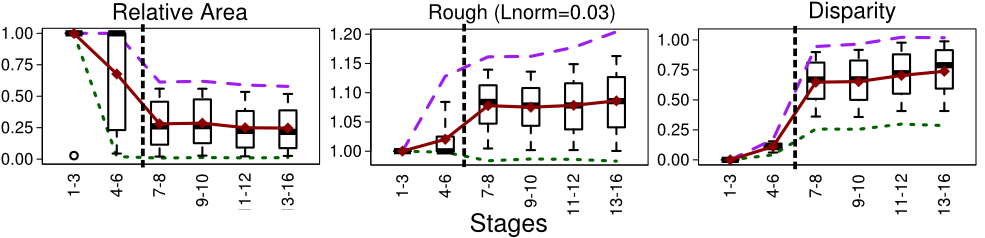
\includegraphics[width=\textwidth]{./Images/Art-I/3_measures.png}
  \centering
  \caption{\textbf{Measures in \textit{Drosophila}}.Distribution plot of the relative area of expression (left), roughness (center) and disparity (right) for all genes in each stage. Diamonds represent the mean, boxes the Inter Quartile Range (IQR). Whiskers 10 and 90 percentiles. Dashed line represents the max values and dotted line the min values (mean of the last and first decile, respectively). Stages on the x-axis, vertical dashed line represents gastrulation entry.
	\nomenclature{IQR}{Inter Quartile Range} 
  }
  \label{fig:Art-I-3measures}
\end{figure}
%%%%%%%%%%%%%%%%%%%%%%%%%%%%%%%%%%%%%%%%%%%%%%%%%%%%%%%%%%%%%%%%%%%%%%%%%%%%%%%%%%%%%%%%%%%%%%%%%%%%%%%%%%%%%%

\subsubsection{Main spatio-temporal profiles in \textit{Drosophila}}
%With a time series cluster analysis \citep{Ernst2006} of the relative area of expression, 
Using a time series cluster analys, I found the eight main spatio-temporal profiles of gene expression in the embryonic development of \textit{Drosophila} (study I, Fig. 5). As expected, the most common profile (n=297 genes) follows the global profile of non-linear decrease in the first stages (I, Fig 5).
%
I also found both linear increase and decrease profiles and a "hill-like" profile (initial increase and further decrease with the higher values at stage 7-8)
%
The linear decrease profile (n=167 genes) was enriched with "mitotic cell cycle" (GO:0000278), "RNA processing" (GO:0006396) and "chromatin modification" (GO:0016568) GOterm genes, highlighting biological processes that first are present in the whole embryo and become more and more restricted in space as development proceeds.
%discussion
The "mitotic cell cycle" term, for example, most likely relates to the fast mitotic cycles in the earliest embryo. During stage 1-3 nine fast and synchronic mitotic divisions take place in the entire embryo, then in stage 4-6 mitotic divisions 10-13 occur more slowly, almost synchronically. The 14th cycle, zygotically controlled, is long and of different durations in the embryo.

With a temporal co-expression cluster analysis using microarray data through the life cycle of \textit{D. melanogaster}, \citet{Arbeitman2002} found that most cell cycle genes were expressed at high levels during the first 12h, but only a few are expressed at high level thereafter.
My analysis is consistent with this, as I found that the profile of linear decrease (I, Fig. 5A) is enriched with such genes. In this sense, this study is complementary to Arbeitman et al., and adds the spatial dimension to their temporal expression profiles.


%%%%%%%%%%%%%%%%%%%%%%%%%%%%%%%%%%%%%%%%%%%%%%%%%%%%%%%%%%%%%%%%%%%%%%%%%%%%%%%%%%%%%
\subsection{Disparity}
%objective
As the relative area (or volume) of expression informs on how genes are expressed in progressively smaller regions in the embryo, the disparity measure can inform about how different regions of the embryo express increasingly different combinations of genes.
%Therefore, both measures reflect slightly different aspects of complexity that are independent from each other. A decrease in the volume of expression of genes does not necessarily imply an increase in spatial disparity: genes could decrease their volume of expression but end up restricted to the same parts of the embryo. 
%If the majority of genes would be expressed ubiquitously (this is large volume), however, then the mean disparity between its regions would be necessarily low. 
%
%results
My results show that in each species, the global disparity pattern is similar to the relative area or volume patterns.
Therefore, in \textit{Drosophila} the disparity increases mostly in the transition from the maternal to early gastrula and in Ciona this major change occurs after gastrulation.

%%%%%%%%%%%%%%%%%%%%%%%%%%%%%%%%%%%%%%%%%%%%%%%%%%%%%%%%%%%%%%%%%%%%%%%%%%%%%%%%%%%%%%%%%%%%%%%%%%%%%%%%%%%%%%
\begin{figure}[b]
  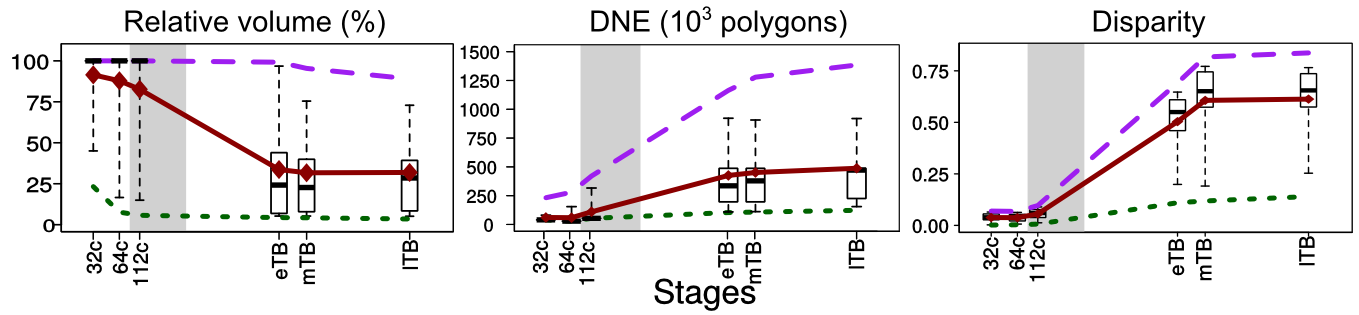
\includegraphics[width=\textwidth]{./Images/Art-II/3_measures_nostars.png}
  \centering
  \caption{\textbf{Measures in \textit{Ciona}.} Distribution plot of the relative volume of expression (left), DNE (center) and disparity (right) for all genes in each stage. Diamonds represent the mean, boxes the IQR. Whiskers 10 and 90 percentiles. Dashed line represents the max values and dotted line the min values (mean of the last and first decile, respectively). Stages on the X-axis (s32c, 32-cells; s64c, 64-cells; s112c, 112-cells; eTB, early tailbud; mTB, mid tailbud; lTB, late tailbud). Grey area represents gastrulation period.}
  \label{fig:Art-II-3measures}
\end{figure}
%%%%%%%%%%%%%%%%%%%%%%%%%%%%%%%%%%%%%%%%%%%%%%%%%%%%%%%%%%%%%%%%%%%%%%%%%%%%%%%%%%%%%%%%%%%%%%%%%%%%%%%%%%%%%%

% discussion
It is important to notice that these measures should not necessarily correlate (see section \ref{measures_relations}.
%
In \textit{Ciona} I found an example of a case when there is no perfect correspondence between the relative volume and the disparity of expression: disparity increased significantly between early to mid-tailbud stages but no significant differences between the relative volume of expression of these stages were found (II, Fig. 3A).
This means that, on average, genes are expressed in a similar number of tissues in these stages, but in the mid tailbud the combination of genes expressed in these tissues are more different between each other.

This shows that the disparity measure is useful specially when is complemented with the relative area (or volume) measure to describe the compartmentalization of the embryo.

%%%%%%%%%%%%%%%%%%%%%%%%%%%%%%%%%%%%%%%%%%%%%%%%%%%%%%%%%%%%%%%%%%%%%%%%%%%%%%%%%%%%% 

\subsection{The leading role of TFs and GFs (and other signalling molecules)}

%%%%%%%%%% articulo 1
%objective
%I wanted the test in both species if TFs and GFs showed an earlier compartmentalization or greater disparity when compared to the rest of the genes. This would be expected from their allegedly leading role in early pattern formation.

%results 1
Using a GOterm analysis in \textit{Drosophila}, I found that TFs (GO:0003700) and GFs (GO:0008083) showed smaller relative area of expression that the rest of genes in the blastoderm stage (Fig. \ref{fig:Art-I-3measures}).
	\nomenclature{GF}{Growth Factor}
	\nomenclature{KW}{Kruskal-Wallis test}
%
The TFs are also expressed in smaller areas than the rest of the genes in all subsequent stages, while the GFs are expressed in smaller areas at the blastoderm (stage 4-6) and extended germ band stages (stage 9-10 and 11-12) (I, Fig.4). In the blastoderm stage the disparity of the regions based only on the TFs is much greater than the one based on all the genes ((KW pvalue $<0.001$, see study I) confirming that these genes account for a large portion of the diversity of gene expression patterns in the blastoderm stage.

%discussion 1
These results are consistent with a previous study of TFs expression during \textit{Drosophila} embryogenesis done by \citet{Hammonds2013}.
They made an extensive analysis of TFs expression using manual annotation of gene expression based on an anatomical controlled vocabulary and classifying every gene as ubiquitous, patterned, ubiquitous-patterned, or maternal (from the BDGP database; \citealp{Tomancak2007}).
They found that the fraction of TFs expressed in a restricted pattern (assigned to a tissue) was higher, when compared to other genes, in all zygotic stages with the exception of the stage 13-16. 
The results I show for stages 4-6, 7-8, 9-10 and 11-12 are consistent with Hammonds et al., as the higher proportion of the TF genes showing a restricted or tissue-specific expression pattern would imply that TFs are expressed in smaller areas in the embryo. For the 13-16 stage, contrary to these authors, I showed that the TFs are highly compartmentalized. This might indicate a limitation of the annotation method used by Hammonds et al., to capture the high spatial compartmentalization of the TFs in this stage.

%%results & discusion 2
%

%%%%%%%%%%%%%%%% articulo 2 
%objective
In \textit{Ciona}, I performed a similar analysis using the categorization of TFs and signaling molecules (SIGs) made by \citet{Imai2004}.
SIGs consist of genes of receptor tyrosine kinase (RTK) pathways such as FGFs and intracellular signalling molecules such as MAPK, Notch, Wnt, TGF$\beta$, Hedgehog and genes in the JAK/STAT pathways \citep{Imai2004}. 

	\nomenclature{SIGs}{Signaling molecules}
	\nomenclature{RTK}{receptor tyrosine kinase}

%results 1
As expected, TFs volume of expression decreased faster than non-TFs. The TFs showed lower volume of expression in the 64-cell and 112-cell stages (II, Fig. 3B). 
The results are similar for maternal and zygotic genes (maternal/zygotic classification based on \citealp{Matsuoka2013}; II,Fig. S1). I then compared TF families and found that six TF families showed lower relative volume in the early gastrula (BZIP, T-box, bHLH, HMG, Nuclear Receptor, and `Other-TFs') but only T-box genes showed a lower relative volume from the 32-cell stage until gastrula (II,Fig. S2). 

%discussion 1
The results obtained for the T-box gene family (conserved in metazoan and several non-metazoan lineages \citep{Sebe-Pedros2013}) are consistent with the known important role these genes have in diverse metazoan species early cell fate specification (reviewed in: \citealp{Papaioannou2014,Showell2004}.
Examples of T-box genes in \textit{Ciona} are Tbx6 and \textit{brachyury}, crucial for muscle tissue formation \citep{Mitani1999,Nishida2005} and for notochord specification \citep{Yasuo1998}, respectively.
%results 2
I also found that the SIGs showed significant lower relative volume of expression than the rest of the genes in the 32-cell, 64-cell, and 112-cell stages (II, Fig. 3B).
Specifically, in the 64-cell stage RTK-MAPK, Wnt and TGF$\beta$ families showed significant higher disparity in the 64 cells stage, suggesting a predominant role of these pathways in the patterning of the embryo at this stage. 
%discussion2
This is consistent with known short range induction events by nodal and various FGFs, which are part of the TGF$\beta$ and RTK-MAPK signalling pathways, respectively \citep{Lemaire2008}.

%general discussion? (X)

In general, the fact that in these two species that display a very different development TFs and GFs (or SIGs in the case of \textit{Ciona}) are more compartmentalized than the rest of the genes precisely in the stage before entering gastrulation, is consistent with these genes having a special role in pattern formation and compartmentalization.
Therefore, these results support the hypothesis of the leading role of TFs and GFs in driving pattern formation and compartmentalization in the early embryo.

%%%%%%%%%%%%%%%%%%%%%%%%%%%%%%%%%%%%%%%%%%%%%%%%%%%%%%%%%%%%%%%%%%%%%%%%%%%%%%%%%%%%% 
%%%%%%%%%%%%%%%%%%%%%%%%%%%%%%%%%%%%%%%%%%%%%%%%%%%%%%%%%%%%%%%%%%%%%%%%%%%%%%%%%%%%% 
\subsection{2D and 3D roughness analyses}
%% objective
%
%I wanted to test the hypothesis of gene expression spatial patterns becoming more complex during development.
%In here, with gene expression spatial pattern I mean the spatial distribution of the cells or tissues expressing a specific gene. 
%
%Considering that I had information in 2D in \textit{Drosophila} and in 3D in \textit{Ciona}, it was necessary to apply a specific method for each species.
As explained in the methods, in order to test the hypothesis of gene expression spatial patterns becoming more complex during development, I developed a I developed a "roughness" measure \citep{Salvador-Martinez2015} for \textit{Drosophila}, which accounts for the curvature of the contour in a 2D gene expression pattern, normalizing it with the contour of a circle of the same perimeter.
In \textit{Ciona}, I applied a similar measure of curvature in 3D, called `Dirichlet normal energy' (DNE), which quantifies the deviation of a surface from being planar \citep{Bunn2011}. To improve the readability of the text,  I will refer to the roughness measure in \textit{Drosophila} as 2D roughness and to the DNE measured used in \textit{Ciona} as 3D roughness.
	\nomenclature{DNE}{Dirichlet Normal Energy}
Both measures not only inform about the overall imbrication or convolution of the shape of a gene expression pattern, but also do it at different spatial scales.
%
%In the following paragraphs, to improve the readability of the text,  I will refer to the roughness measure implemented in \textit{Drosophila} as 2D roughness and to the DNE measured used in \textit{Ciona} as 3D roughness.
%

%results
The results show that both 2D and 3D roughness increase in a non-linear way during development.
As with the compartmentalization and disparity, the difference between species is where the major change is found. 

%drosophila
In \textit{Drosophila}, the major change is found in the transition from the blastoderm to the early gastrula (Fig. \ref{fig:Art-I-3measures}).
When analysing the maximal values (mean of the last decile) it can be seen that they increase initially in the pre-gastrula, reach a stationary phase at mid-embryogenesis and finally increase in the last stages. 
The maximal values are informative about the overall morphological spatial complexity of the embryo in a given stage.
When comparing roughness at different spatial scales (I, Methods), I found that in the last three stages the roughness values are significantly higher at smaller spatial scales is significantly higher that at the higher spatial scales.(Fig. S2 in article I). 

%Ciona
In Ciona, the 3D roughness increase throughout development (II, Fig. 5), with the major change between the 112-cell and the early tailbud (Fig. \ref{fig:Art-II-3measures})  
The max (mean of the last decile) values increase substantially already between the 64 and 112 cells stages (with 1000 and 10000 polygonal faces), while the min values (mean of the first decile) remain practically constant during development, showing that the most complex patterns in each stage get increase their DNE value but there is always a proportion of very simple expression pattern.
Also, I found that at low spatial scales (1000 and 10000 polygons per mesh; II, Fig. 5) I found that the mean DNE of the late tailbud is higher than at the mid tailbud (one-way ANOVA pvals < 0.05).
	\nomenclature{ANOVA}{Analysis of Variance}

%% general discussion
In summary, this results show that the complexity of distribution in space of cells/tissues expressing a gene increases through development, and that these complexity (measured with the 2D and 3D roughness) increase in both \textit{Ciona} and \textit{Drosophila} in a similar way than the other two measures, compartmentalization and disparity.
Also, by analysing the roughness at different scales, I found compelling evidence that complexity may be increasing not only through all the development but also that it does at finer spatial scales over time.

%%%%%%%%%%%%%%%%%%%%%%%%%%%%%%%%%%%%%%%%%%%%%%%%%%%%%%%%%%%%%%%%%%%%%%%%%%%%%%%%%%%%% 
\subsection{Synexpression territories}
%objective
%I wanted to explore in both species the relative degree of similarities between different parts of the embryo within and between different developmental stages.
%
%To do this I used two different approaches, based on the differences between the databases I used for each species.
%In \textit{Drosophila} I used the polar regions with which I computationally divided the embryo. In \textit{Ciona}, I took advantage of the available information at the individual cell/tissue.  

In both species I used a clustering algorithm to produce dendrogram representing the relative degrees of similarities between all regions of different stages at the same time (Fig. \ref{fig:Art-I-territories} and Fig. \ref{fig:Art-II-territories}).
I will refer to the regions that clustered together as "synexpression territories" (STs).
	\nomenclature{ST}{Synexpression territories}

%%%%%%%%%% drosophila
In \textit{Drosophila}, after cutting the dendrogram at a specific threshold and filtering out STs with less than 50 genes expressed with a minimum specificity (see methods in I for a detailed description), 30 STs were selected for further analyses (Fig. \ref{fig:Art-I-territories} B).

%Finally, I grouped the STs in eight `meta-territories' to analyse how the different STs relate between them.
Finally, I grouped the STs in eight `meta-territories', as I wanted not only to see how the regions in the embryo formed different STs, but also how different STs cluster with each other, as this is informative of the degree of differentiation between stages. If STs cluster with other STs in the same stage, it would mean that the majority of genes change their expression in a similar way over time independently of where they are.
If STs cluster with other STs in the same part of the embryo in successive stages, it would mean that this part of the embryo has expression dynamics independent from other parts of the embryo, which would be expected in already differentiated cells/tissues.

%%%%%%%%%%%%%%%%%%%%%%%%%%%%%%%%%%%%%%%%%%%%%%%%%%%%%%%%%%%%%%%%%%%%%%%%%%%%%%%%%%%%%%%%%%%%%%%%%%%%%%%%%%%%%%
\begin{figure}[ht]
  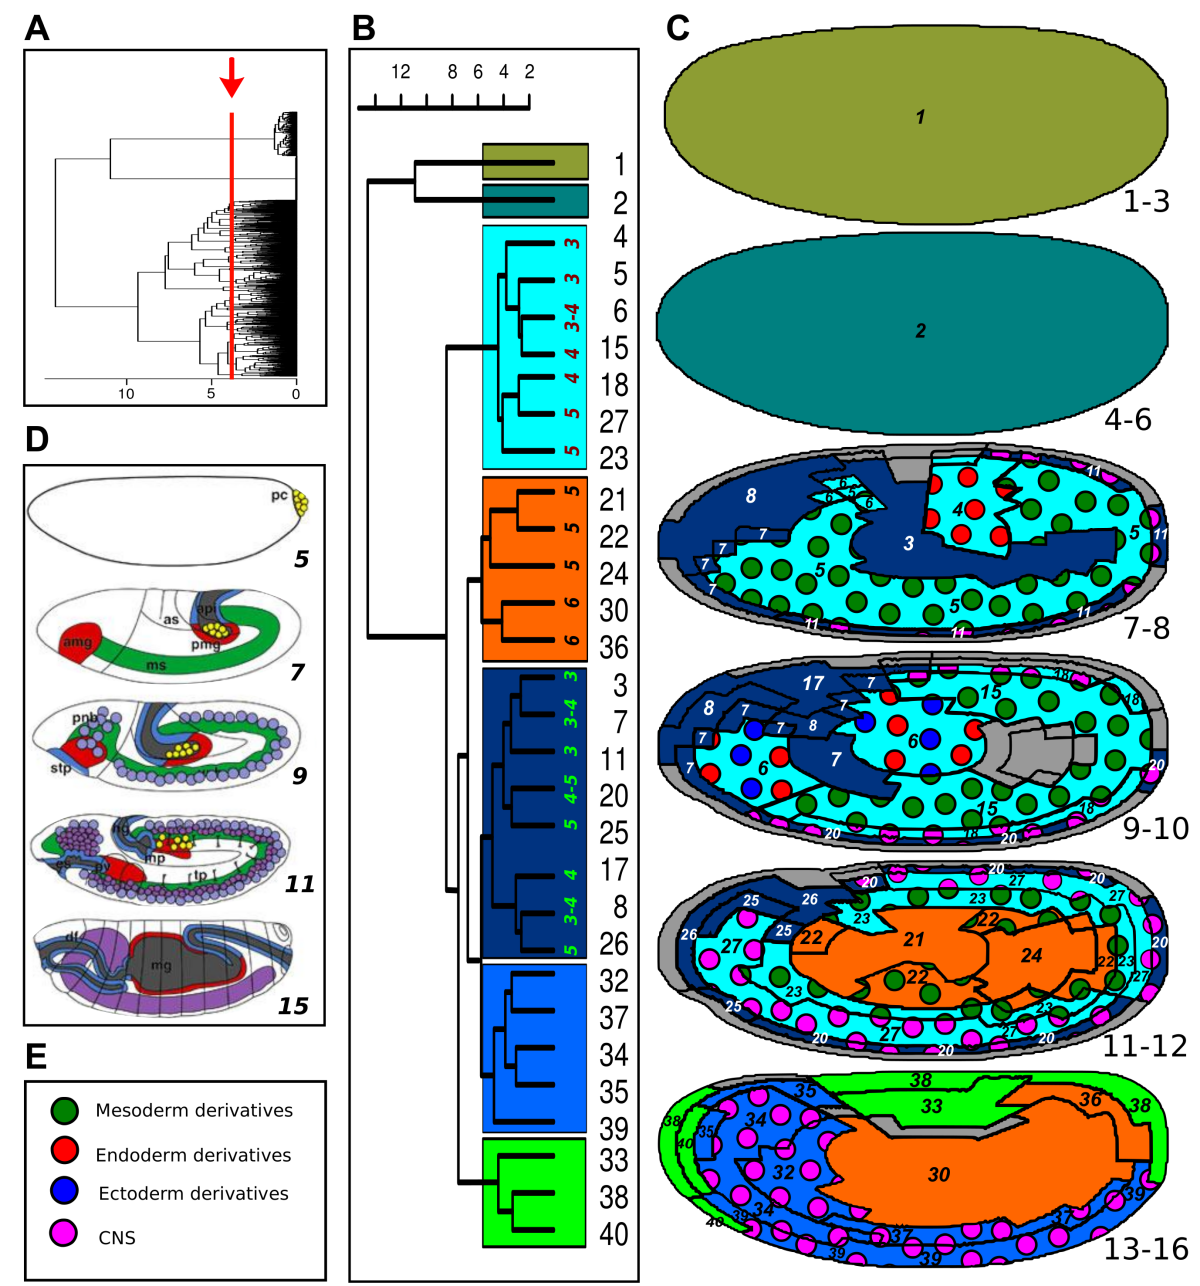
\includegraphics[width=0.65\textwidth]{./Images/Art-I/territories.png}
  \centering
  \caption{Synexpression territories (ST). (A) Dendrogram produced by hierarchical clustering on a similarity matrix (pearson's correlation) of all the embryo regions of the six stages. Red line shows the cut-off to produce 40 STs. (B) Dendrogram reconstructed using only territories with at least 50 genes with a minimum specificity (I, methods). The coloured boxes show the main branches of the dendrogram. The number indicated inside the boxes represent the stages each ST corresponds to (3 is stage 7-8, 4 is stage 9-10, 5 is stage 11-12 and 6 is stage 13-16). The ST number is at the right. (C) STs mapped onto the embryo. Gray regions have less than 50 genes expressed. Background color refers to which `meta-territory' (in B) each ST is part of. Coloured circles represent GOterm enrichment of a specific tissue/germ layer derivative (shown in E). Stages in the lower-left part of each embryo. From stage 7-8, the ST number (as in B) is indicated. (D) Hartenstein's embryo schemes \citep{Hartenstein1993} with their respective stages in the left upper part. (E) Colour code of specific tissue/germ layer derivative used in C.)}
  \label{fig:Art-I-territories}
\end{figure}
%%%%%%%%%%%%%%%%%%%%%%%%%%%%%%%%%%%%%%%%%%%%%%%%%%%%%%%%%%%%%%%%%%%%%%%%%%%%%%%%%%%%%%%%%%%%%%%%%%%%%%%%%%%%%%

%results
The results show that stages 1-3 and 4-6 each one form a ST. If a cut-off is selected so that stage 4-6 is divided in four sub-territories (I,Fig. S3) the embryo splits in four parts: anterior, posterior, dorsal and ventral.
This correspond to a nearly Cartesian system one could expect from the two signalling systems known in the earliest patterning in \textit{Drosophila} (the A/V and D/V signalling cascades; \citep{Gilbert2014}).
%
The STs seem to coincide with the known embryo fate map (see Fig. \ref{fig:Art-I-territories} D; \citealp{Hartenstein1993}) and many of them are enriched with GOterms that coincide with their expected fate.
For example, in stage 7-8 (just after gastrulation) there is a ST that corresponds spatially with the germband and is enriched with mesodermal GOterms (Fig. Fig. \ref{fig:Art-I-territories} C).

Two meta-territories appear in the last stage (light blue and green, Fig. \ref{fig:Art-I-territories} C), which suggests that the tissues/organs related to those STs differentiate quite late.
%
%% discussion
One of these meta-territories is enriched with terms related to epidermis such as cuticle development ("chitin catabolic process" [GO:0006032] and "cuticle development" [GO:0042335] STs 33 and 38), which coincides with cuticle deposition by epithelial cells during stage 16 \citep{Ostrowski2002}.
%
The other meta-territory corresponds spatially with the CNS of the embryo and is indeed enriched with CNS GO-terms.
The CNS territory is enriched with GOterms like "dendrite morphogenesis" (GO:0048813) and "axon guidance" (GO:0007411). 
	\nomenclature{CNS}{Central Nervous System}

%%%%%%%%%%%%%%%%%%%%%%%%%%%%%%%%%%%%%%%%%%%%%%%%%%%%%%%%%%%%%%%%%%%%%%%%%%%%%%%%%%%%%%%%%
\begin{figure}[ht]
  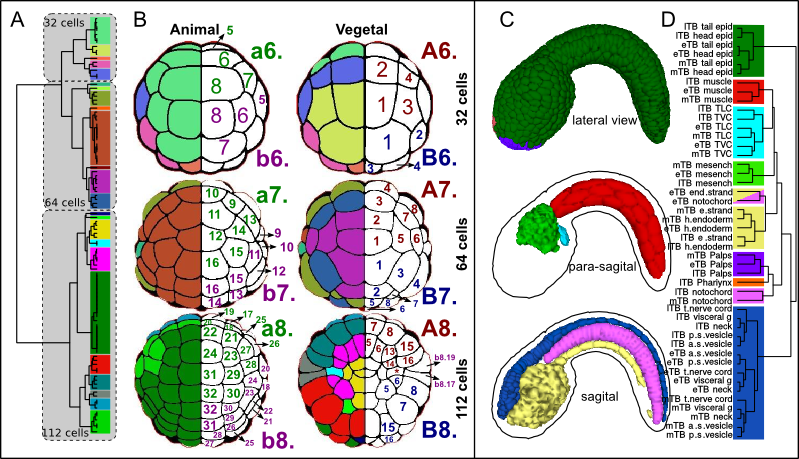
\includegraphics[width=\textwidth]{./Images/Art-II/territories.png}
  \centering
  \caption{Ciona synexpression territories. 
  (A) Dendrogram produced by hierarchical clustering of cells in 32-cell, 64-cell and 112-cell stages. Dashed boxes show that STs cluster by stage. Coloured boxes show the cut-off to produce 24 STs.
  (B) Names of cells (Conklin nomenclature; \citealp{Conklin1905}) indicated with a prefix shown at right. STs in the 32 cells, 64 cells and 112 cells stages (top, middle and bottom, respectively). Colour refers to which ST of the dendrogram (in A) each cell is part of. Animal view based on \citet{Nicol1988} and vegetal view based on \citet{Cole2004a}. The cell marked with a star (*) is the A7.6 cell, that in this analysis represents their descendant cells (A8.11 and A8.12).
  C) Dendrogram produced by hierarchical clustering of tissues in early, mid and late tailbud stages. The coloured boxes show the cutoff to produce 10 STs. (D) STs in the tailbud stages shown in a lateral, para-sagital and sagital views of a mid tailbud 3D embryo model (from \citealp{Nakamura2012}). Colour refers to which ST of the dendrogram (in C) each tissue is part of.
}
  \label{fig:Art-II-territories}
\end{figure}
%%%%%%%%%%%%%%%%%%%%%%%%%%%%%%%%%%%%%%%%%%%%%%%%%%%%%%%%%%%%%%%%%%%%%%%%%%%%%%%%%%%%%%%%%%%%

In \textit{Ciona}, because gene expression information in tailbud stages is based on tissues and not on individual cells as the early stages, I analysed the STs of these stages separately (II, Methods). 

%results
If in the early stages, three "meta-territories" are formed, each one would correspond to one stage, i.e., STs in early stages cluster by stage.
Thus, even if at the first three stages a high proportion of blastomeres express a nearly unique combination of transcriptional factors \citep{Imai2006}, the bulk change in gene expression is common to all blastomeres. Within each early stage, STs coincides very well with the know fate map (II, Fig 6A; II, Fig. S8), with some exceptions I will describe in the next subsection.
%
In contrast, in tailbud stages practically all STs cluster by tissue/cell type, which indicates that the in early tailbud, most tissues are already quite differentiated.
This is consistent with studies analysing these stages at the level of individual or small sets of genes \citep{Corbo1997,DiGregorio1999}.

%discussion 2
This analysis in the early stages is similar to the one made by \citet{Imai2006}, who used the expression profile of 53 zygotically TFs in single cells in the 16, 32, 64, and 112-cell stages, to perform a hierarchical clustering (for each stage separately). 
It is different in two aspects: I performed the clustering using the blastomeres of different stages and my analysis is not restricted to TFs. As I said previously, using various stages is informative of the overall differentiation process and can be used to discern between differentiation scenarios, as the differences between early and tailbud stages I found here.

%%% general discussion
\subsection{General discussion}

% discussion
The difference in the timing of the major change on the complexity measures between species must relate to differences in their specific development.
The earlier compartmentalization of \textit{Drosophila} is most probably due to its derived early development, namely, the syncytial blastoderm. 
During the blastoderm stage, approximately 4,000 cell nuclei can "communicate" with each other only by TFs \citep{Jaeger2011}. The direct cross regulation of gene expression facilitates a rapid and highly dynamic process which seems to be responsible for the early spatial restriction of a great proportion of developmental genes.
It could be therefore expected that these early increase in complexity in \textit{Drosophila} would be shared by all insects with a syncitial blastoderm stage. Also, it could be that the early increase in complexity might be affected by the number of cell divisions that occur until the blastoderm is cellularized. It is known that \textit{Drosophila} cellularizes relatively late (so there is more time for patterning within the syncitial bastoderm). In contrast, the desert locust (\textit{Schistocerca gregaria}) cellularization occurs very early, even before the formation of the blastoderm \citep{Ho1997}.

In contrast,  \textit{Ciona}'s early embryonic patterning is based on maternal determinants and signalling events mostly between neighbouring cells \citep{Lemaire2009}, which act in a combinatorial way \citep{Hudson2007} to establish a unique TF combination in more than half of the blastomere pairs before gastrulation \citep{Imai2006} determining most of their fates.
Thus, even when in \textit{Ciona} most of the cell fates are already determined (by the specific combination of a fraction of TFs) and the embryo can be said to be already highly compartmentalized, this is not evident at the global level of gene expression, which I am measuring here.
Therefore, the "delay" of compartmentalization observed in \textit{Ciona} could be explained by the relatively slower process of signal transduction (as in \textit{Ciona}) compared to the gap gene network (in \textit{Drosophila}).

Another main difference between species is that, based on the synexpression terriories analysis the the differentiation process in \textit{Drosophila} seems to continue throughout whole embryogenesis (as new STs were formed until the last stage I analysed) and different organs differentiate at different developmental times.
In contrast, the \textit{Ciona} embryo seems to be already genetically differentiated at the early tailbud (as the STs of all the tissues in the tailbud stages cluster together) so the last embryo stages consist only of moderate morphogenetic movements (mainly cell elongation; \citealp{Hotta2007}).
Therefore, the ST analysis is a valuable tool, based on differential gene expression, to get a global perspective on the local differentiation of the embryo.